\documentclass{article}
\usepackage[margin=0.75in]{geometry}
\usepackage{enumitem}
\usepackage{setspace}
\usepackage{amsmath}
\usepackage{amssymb}
\usepackage{physics}
\usepackage{relsize}
\usepackage{graphicx}

\title{CS 143 Homework 3}
\date{2/4/2021}
\author{Jiaping Zeng}

\begin{document}
\setstretch{1.35}
\maketitle

\begin{enumerate}
    \item \begin{enumerate}
              \item As shown below:
                    \begin{center}
                        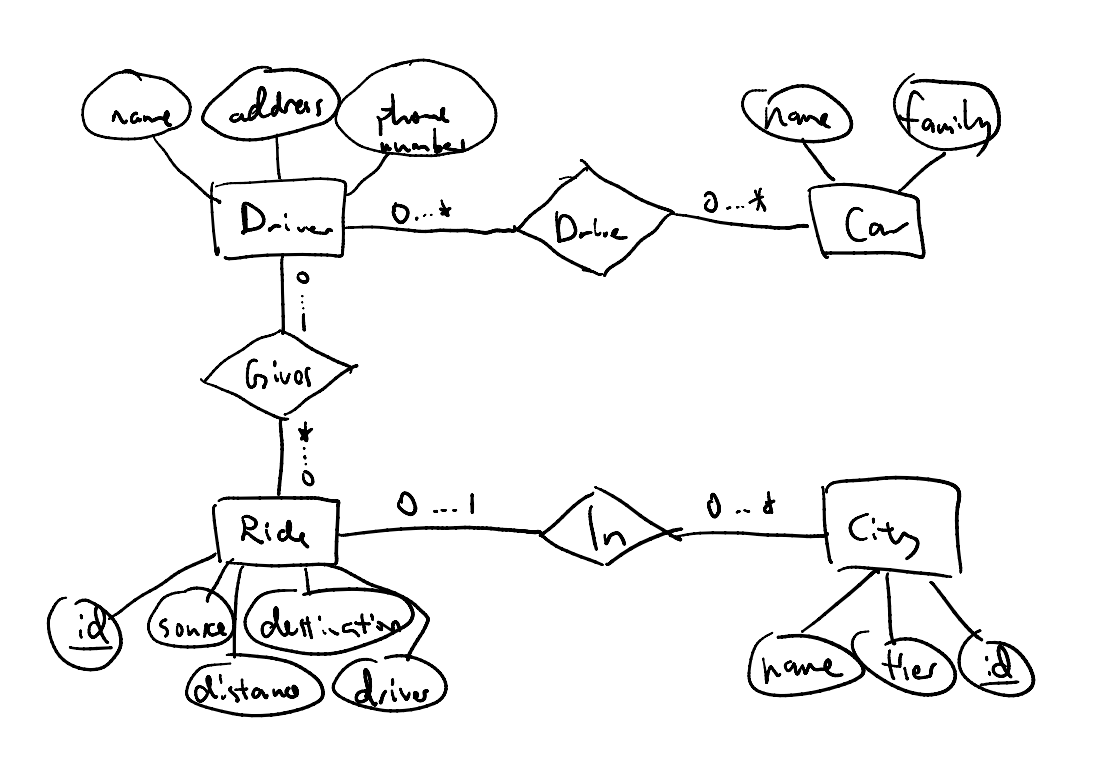
\includegraphics[width=6in]{1a.png}
                    \end{center}
              \item CREATE TABLE Driver(name VARCHAR(20), address VARCHAR(100), phone VARCHAR(20));\\CREATE TABLE Car(name VARCHAR(20), family VARCHAR(20));\\CREATE TABLE City(name VARCHAR(20), tier INT, id INT, PRIMARY KEY(id));\\CREATE TABLE Ride(id INT, source VARCHAR(20), destination VARCHAR(20), distance INT, driver VARCHAR(20), PRIMARY KEY(id));
          \end{enumerate}
    \item As shown below:
          \begin{center}
              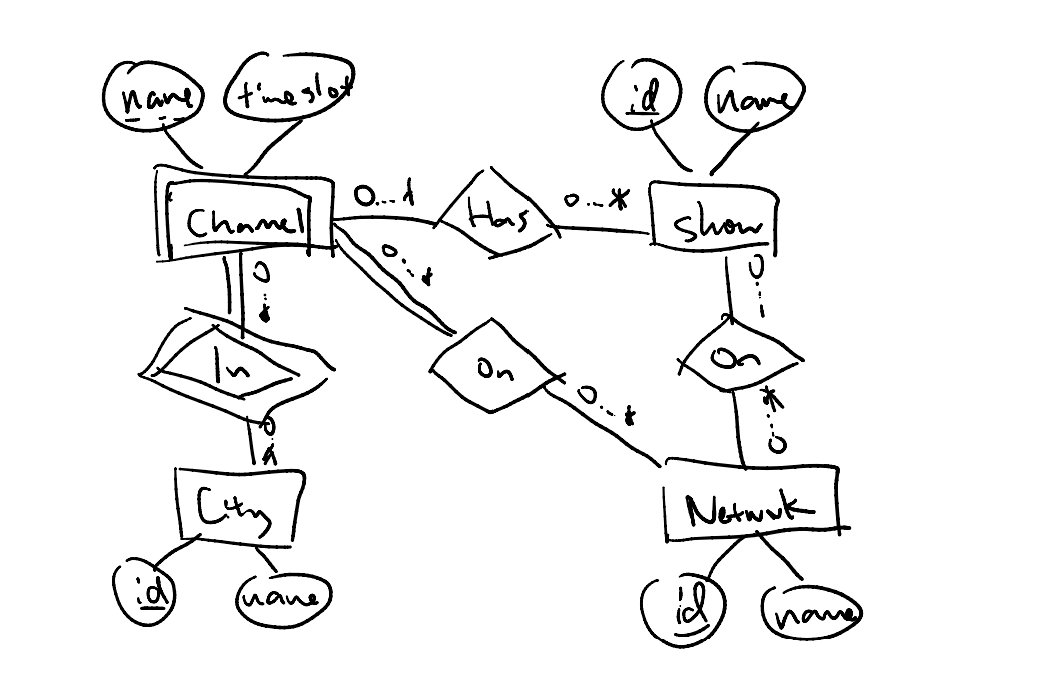
\includegraphics[width=6in]{2.png}
          \end{center}
    \item Programmer(\underline{id},name,leader\_id)\\Team(\underline{leader\_id},)\\TeamLeader(\underline{id},team\_name)\\Project(\underline{id},leader\_id)
    \item Yes because $A\rightarrow B\rightarrow D$, then with $A\rightarrow D$ we have $A\rightarrow CD\rightarrow E$. Therefore $A\rightarrow DE$ so the decomposition is lossless.
    \item $BC\rightarrow A$, $AC\rightarrow B$.
    \item \begin{enumerate}
              \item $sid\rightarrow (dept,cnum)$ and $(dept,cnum)\rightarrow sid$ would indicate an one-to-one relationship.
              \item $(dept,cnum)\rightarrow sid$ would indicate a many-to-one relationship.
          \end{enumerate}
    \item \begin{enumerate}
              \item Yes because $A\rightarrow B\rightarrow D$, then $A\rightarrow CD\rightarrow E$ so $A\rightarrow BCDE$.
              \item Yes because $B\rightarrow D$ then $CD\rightarrow E$ and $E\rightarrow A$, so $BC\rightarrow ADE$.
          \end{enumerate}
    \item No because $F$ cannot be determined so we would need $(A,F)$ as key, so all the funcitonal dependencies fail the BCNF conditions. It can be normalized into a set of relations as follows:\\$R_0(A,B,C): A\rightarrow BC$\\$R_1(B,D):B\rightarrow D$\\$R_2(C,E):C\rightarrow E$\\$R_3(A,F):$ (none)
\end{enumerate}
\end{document}